\documentclass{beamer}
\usetheme{metropolis}           % Use metropolis theme
\title{Gaussian Processes}
\date{\today}
\author{Nipun Batra}
\institute{IIT Gandhinagar}
\begin{document}
  \maketitle
  
  
  
\section{Gaussian Distribution}
  \begin{frame}{1d Gaussian Scatter Plot}
    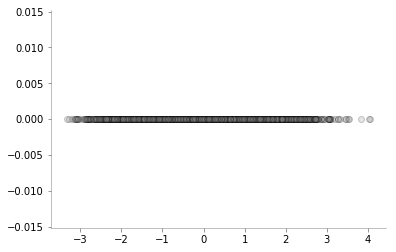
\includegraphics[width=\textwidth]{gp/1d-lineplot}
  \end{frame}

  \begin{frame}{1d Gaussian Histogram}
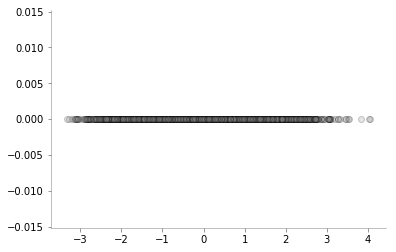
\includegraphics[width=\textwidth]{gp/1d-lineplot}
\end{frame}

  \begin{frame}{Varying 1d Gaussian Variance}
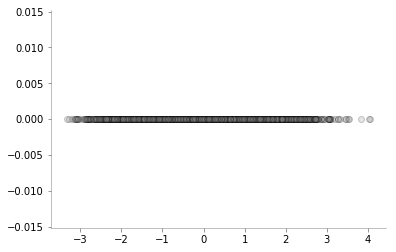
\includegraphics[width=\textwidth]{gp/1d-lineplot}
\end{frame}

\begin{frame}{Bi-variate Gaussian}
$$
\begin{pmatrix}
X_1 \\
X_2
\end{pmatrix}  \sim \mathcal{N} \left( \begin{pmatrix}
\mu_1 \\
\mu_2
\end{pmatrix} , \begin{pmatrix}
a &\rho \\
\rho & b
\end{pmatrix} \right)
$$
\end{frame}


\begin{frame}{Cholesky Decompostion I}
\begin{align*}
\mathbf{A} = \mathbf{L L}^T
\end{align*}
where L is a real lower triangular matrix.


We can thus re-write the posterior mean and covariance as:

\begin{align*}
p(y_*|X_*, X, y) \sim \mathcal{N}(\mu', \Sigma') \\
K = LL^T \\
\end{align*}
\end{frame}

\begin{frame}{Cholesky Decomposition II}
\begin{align*}
\alpha = K^{-1}(x-\mu) \\
or, \alpha = {LL^T}^{-1}(x-\mu) \\
or, \alpha = L^{-T}L^{-1}(x-\mu) \\
Let, K^{-1}(x-\mu) = \beta \\
Thus, L^{-T}L^{-1}(x-\mu) = \beta \\
Let, L^{-1}(x-\mu) = \gamma\\
Thus, L\gamma = x-\mu \\
Thus, \gamma = L \setminus (x-\mu)\\\
Thus, \alpha = L^{T} \setminus (L \setminus (x-\mu))
\end{align*}

\end{frame}
\end{document}